\documentclass{article}
\input{preamble}

\title{Working notes}
\author{Corey Jones, Scott Morrison, David Penneys}


\begin{document}
\maketitle


We define a truncated tensor product $\boxtimes$ of ATLJ modules, which is the usual tensor product, modulo the relations that
any closed diagram passes through a string, and
the $2\pi$ rotation acts identically.

Observe that if $V$ and $W$ are sub-ATLJ modules of a evaluable planar algebra $\cP_\bullet$, there is an ATLJ homomorphism $V \boxtimes W \to \cP_\bullet$, because the additional relations we impose in the truncated tensor product automatically hold in an evaluable planar algebra.

We now aim to completely describe the decomposition of this truncated tensor product into irreducibles. 
To prepare for this, we need some discussion of lowest weight vectors in ATLJ modules.

Recall the isomorphism classes of minimal idempotents in the Temperley-Lieb-Jones algebra are the Jones-Wenzl idempotents $f^{(n)}$. 
It is convenient to pass to the idempotent completion, and consider the TLJ algebra as a semisimple category with simple objects $f^{(n)}$. 
The annular Temperley-Lieb-Jones category contains as a full subcategory the category with objects \nn{circle with one marked point, labelled by fn} which we call the tube category $\cT$. This inclusion is a Morita equivalence, giving an equivalence between $\Rep(ATLJ)$ and $\Rep(\cT)$. This is explained in \cite[Proposition 3.5]{1502.06543}.

\nn{Some remarks about what irreps of $\cT$ look like, and that there's only one annular consequence of the generator in each higher weight space.}

Suppose $\cV$ is some $\cT$ module.

\begin{lem}
When $\delta>2$, the lowest weight vectors in $\cV_m$ are the kernel of $\cL_m : \cV_m \to \cV_m$
$$
\cL_m = \mathfig{0.2}{LowestWeightTangle}.
$$
\end{lem}
\begin{proof}
First, it is clear that the lowest weight vectors are the kernel of $a$, where $$\mathfig{0.2}{LoweringOperator}.$$

Certainly $\ker(a)\subset\ker(\cL_m)$.
To show the other direction, we look at a basis of eigenvectors for $\cL_m$ acting on $\cV_m$ consisting of the new low weights, together with the annular consequences of previous low weights.  
$$
\mathfig{0.4}{PreviousLowWeightsInW}.
$$
By \cite[Proposition 5.3]{1502.06543}, as long as $\delta > 2$, $\cL_m$ has non-zero eigenvalue on the annular consequence.  Therefore only the uncappable vectors can be in the $Ker(\cL_m)$.
\end{proof}

$$\text{if $x>0$}$$

We then define the two operators $\rho, \rho' : \cV_m \to \cV_m$ as
$$
\mathfig{0.3}{CutDownRotation}.
$$


\begin{lem}
The lowest weight vectors with rotational eigenvalue $\omega$ in $\cV_m$ can alternatively be characterized as the solutions of 
\begin{align*}
\rho(v) & = \omega v \\
\rho'(v) & = \omega^{-1} v.
\end{align*}
\end{lem}
\begin{proof}
First we expand the middle Jones-Wenzl idempotent in 
$$
\mathfig{0.3}{RhoRhoPrime}
$$
into a linear combination of Temperley-Lieb-Jones diagrams. 
Only the identity diagram and the diagram
$$
\mathfig{0.2}{JonesProjection}
$$
contribute, and we obtain
$
\rho \circ \rho' = \id_{W_m} - [m-1]/[m] \cL_m
$.
If $v$ is a eigenvector with eigenvalue $\omega$, then $$\rho \circ \rho'(v)=v-[m-1]/[m] \cL_m (v),$$ so $\cL_m(v)=0$, and $v$ is uncappable.
The converse is trivial.
\end{proof}

\begin{defn}
Consider irreducible $\cT$ modules $V^{n_+, \omega_+}$ and $V^{n_-, \omega_-}$, with lowest weight generators $S_+$ and $S_-$. (The use of $\pm$ as a label here has nothing to do with shadings; it's just convenient for our later formulas.) Fix $m\geq 0$ such that $n_+ + n_- + m = 0 \pmod 2$, and define for $0 \leq j \leq \lfloor (m-2)/2 \rfloor$ and $0 \leq i < n_\pm - k_j$ 
\begin{align}
\label{eq:basis-elements}
T^{\pm}_{j,i} & = \mathfig{0.2}{Tpmji}
\end{align}
where $k_j = (n_+ + n_- - m + 2j)/2$.

When $n_-<n_+$, and we connect $S_-$ completely to $S_+$, we have another sequence of elements:
\begin{align}
\label{eq:basis-elements-small}
T^{\pm}_{j,i} & = \mathfig{0.2}{TjiSmall}
\end{align}
\end{defn}

\begin{fact}
A basis for $\left(V^{n_+, \omega_+} \boxtimes V^{n_-, \omega_-}\right)_m$ is given by $\{T^\pm_{i,j}\}$ for $0 \leq j \leq \lfloor (m-2)/2 \rfloor$ and $0 \leq i < (m + n_\pm -  n_\mp - 2j)/2$.
\end{fact}

\begin{lem}
Consider irreducible $\cT$ modules $V^{n_+, \omega_+}$ and $V^{n_-, \omega_-}$, and let $U=V^{n_+, \omega_+} \boxtimes V^{n_-, \omega_-}$.
Let $W_m$ be the space of uncappable vectors in $U_m$.
Then $$\dim(W_m)=\begin{cases} m & \text{if $n_+ + n_- + m = 0 \pmod 2$, and} \\ 0 & \text{otherwise.}\end{cases}$$
\end{lem}
\begin{proof}
Let $\gA_m(S)$ be the space of $\cT$-annular consequences of $S$ in $U_m$.

Assume for now that $n_+ = n_- \pmod 2$, and that $m$ is even. \nn{The other case is similar.}
We use the basis for $U_m$ described above, to count dimensions.
It's now straightforward that $\dim(U_m)=m+\dim(U_{m-2})$, since
$$
U_{m}
=
\gA_m(W_0)\oplus\cdots\oplus \gA_m(W_{m-2})\oplus W_m 
= 
\gA_m(U_{m-2})\oplus W_m
$$
Note that $U_{2}=W_{2}$ since $W_{0}$ is the ``trivial'' representation. 
By induction on $m$, it suffices to show that $\dim(W_{2})=2$.  
This follows from direct computation.
\end{proof}

\begin{thm}
Consider irreducible $\cT$ modules $V^{n_+, \omega_+}$ and $V^{n_-, \omega_-}$, with lowest weight generators $S_+$ and $S_-$.
The truncated tensor product decomposes as
$$
V^{n_+, \omega_+} \boxtimes V^{n_-, \omega_-} 
\iso 
\bigoplus_{\substack{m \geq 0 \\ \text{$m + n_+  + n_-$ is even} \\ \omega^m = 1}} V^{m, \omega},
$$
with low weight generators 
$$
X_{m, \omega} 
= 
\sum_{\pm \in \{+,-\}}
\sum_{j=0}^{\lfloor\frac{m-2}{2}\rfloor}
\sum_{i=0}^{n_\pm-k_j-1} 
(c_{m,\omega})^{\pm}_{j,i} T^\pm_{j,i}
$$
where
$k_j = \frac{n_+ + n_- + 2j - m}{2}$, $T^\pm_{j,i}$ is as defined in Equation \eqref{eq:basis-elements}, and the $(c_{m,\omega})^{\pm}_{j,i}$ are determined by the equations
\begin{align*}
\todo{}
\end{align*}
in the case that $m \leq n_1 + n_2$, and are determined by the equations
\begin{align*}
\todo{}
\end{align*}
in the case that $m > n_1 + n_2$.
\end{thm}
\begin{proof}
We apply $\rho$ to $T^m_{j,i}$ and expand the lower Jones-Wenzl idempotent.
$$
\rho(T^m_{j,i})=
\mathfig{0.2}{RhoTmji}
$$
Certainly the identity term contributes, and the only place we can put a cup on top is the top right.
Because the top right cup will result in an extra strand passing around the bottom of the diagram, no matter where we put a cap along the bottom of the expansion of the Jones-Wenzl idempotent, the total number of strands around the bottom cannot decrease. 
Thus is the terms $T^m_{j',i'}$ which appear in $\rho(T^m_{j,i}))$ can never have $j'<j$.

In general there are four different places the cap could appear along the bottom edge of the Jones-Wenzl idempotent.
$$
\mathfig{0.3}{PositionsOfCaps}
\nn{purple, orange, green, red}
$$
In many special cases, some of these places are not possible. We colour code the terms appearing in the expansion of $\rho(T^m_{j,i})$ according to the position of the cap they correspond to.
A \textcolor{purple}{purple} term corresponds to a cap whose left endpoint attaches  the bundle of $j$ strings at the left \nn{}

\begin{lem}
The coefficient of the following Temperley-Lieb diagram in the Jones-Wenzl idempotent $\jw{m}$ is given by
\begin{align*}
\underset{\in \jw{m}}{\coeff}
\left(
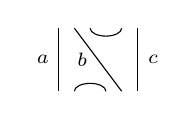
\begin{tikzpicture}[baseline = -.1cm, yscale=-.5]
	\draw (-.5,-.8)--(-.5,.8);
	\draw (-.3,.8) arc (-180:0:.2cm);
	\draw (-.3,-.8)--(.3,.8);
	\draw (-.1,-.8) arc (180:0:.2cm);
	\draw (.5,-.8)--(.5,.8);
	\node at (-.7,0) {{\scriptsize{$a$}}};
	\node at (-.2,0) {{\scriptsize{$b$}}};
	\node at (.7,0) {{\scriptsize{$c$}}};
\end{tikzpicture}
\right)
& =
(-1)^{b+1}\frac{[a+1][c+1]}{[m]}
\end{align*}
{and the coefficient is the same applying any $\bbZ/2\bbZ $-symmetry, and in particular}
\begin{align*}
\underset{\in \jw{m}}{\coeff}
\left(
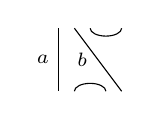
\begin{tikzpicture}[baseline = -.1cm, yscale=-.5]
	\draw (-.5,-.8)--(-.5,.8);
	\draw (-.3,.8) arc (-180:0:.2cm);
	\draw (-.3,-.8)--(.3,.8);
	\draw (-.1,-.8) arc (180:0:.2cm);
	\node at (-.7,0) {{\scriptsize{$a$}}};
	\node at (-.2,0) {{\scriptsize{$b$}}};
    \node at (.2,0) {$\phantom{c}$};
\end{tikzpicture}
\right)
& =
(-1)^{m-a+1}\frac{[a+1]}{[m]}.
\end{align*}
\end{lem}

\begin{itemize}
\item
if you shift $\star$ counterclockwise by one strand, multiply by $\sigma_S$ and switch $\check{}\,$:
$$
\begin{tikzpicture}[baseline = 0cm]
	\draw[thick, unshaded] (0,0) circle (1cm);
	\draw (0,0)--(-10:1cm);
	\draw (30:1cm) --(0,0); 
	\draw (0,0)--(70:1cm);
	\draw (110:1cm) --(0,0); 
	\draw (0,0)--(150:1cm);
	\draw (190:1cm) --(0,0); 
	\draw (0,0)--(230:1cm);
	\draw (310:1cm) --(0,0); 
	\draw[thick, unshaded] (0,0) circle (.4cm);
	\node at (90:.52) {$\star$};
	\node at (0,-.6) {$\cdots$};
	\node at (0,0) {$S$};
	\node at (90:.88) {$\star$};
\end{tikzpicture}
=
\sigma_S\,
\begin{tikzpicture}[baseline = 0cm]
	\draw[thick, unshaded] (0,0) circle (1cm);
	\draw (0,0)--(-10:1cm);
	\draw (30:1cm) --(0,0); 
	\draw (0,0)--(70:1cm);
	\draw (110:1cm) --(0,0); 
	\draw (0,0)--(150:1cm);
	\draw (190:1cm) --(0,0); 
	\draw (0,0)--(230:1cm);
	\draw (310:1cm) --(0,0); 
	\draw[thick, unshaded] (0,0) circle (.4cm);
	\node at (130:.52) {$\star$};
	\node at (0,-.6) {$\cdots$};
	\node at (0,0) {$\check{S}$};
	\node at (90:.88) {$\star$};
\end{tikzpicture}
$$
\item
if you shift $\star$ clockwise by one strand, multiply by $\sigma_S^{-1}$ and switch $\check{}\,$:
$$
\begin{tikzpicture}[baseline = 0cm]
	\draw[thick, unshaded] (0,0) circle (1cm);
	\draw (0,0)--(-10:1cm);
	\draw (30:1cm) --(0,0); 
	\draw (0,0)--(70:1cm);
	\draw (110:1cm) --(0,0); 
	\draw (0,0)--(150:1cm);
	\draw (190:1cm) --(0,0); 
	\draw (0,0)--(230:1cm);
	\draw (310:1cm) --(0,0); 
	\draw[thick, unshaded] (0,0) circle (.4cm);
	\node at (90:.52) {$\star$};
	\node at (0,-.6) {$\cdots$};
	\node at (0,0) {$S$};
	\node at (90:.88) {$\star$};
\end{tikzpicture}
=
\sigma_S^{-1}\,
\begin{tikzpicture}[baseline = 0cm]
	\draw[thick, unshaded] (0,0) circle (1cm);
	\draw (0,0)--(-10:1cm);
	\draw (30:1cm) --(0,0); 
	\draw (0,0)--(70:1cm);
	\draw (110:1cm) --(0,0); 
	\draw (0,0)--(150:1cm);
	\draw (190:1cm) --(0,0); 
	\draw (0,0)--(230:1cm);
	\draw (310:1cm) --(0,0); 
	\draw[thick, unshaded] (0,0) circle (.4cm);
	\node at (50:.52) {$\star$};
	\node at (0,-.6) {$\cdots$};
	\node at (0,0) {$\check{S}$};
	\node at (90:.88) {$\star$};
\end{tikzpicture}
$$
\end{itemize}


When $j=0$, there are either 1 or 2 places for a cap on the bottom, depending on the value of $i$, and the identity term in the Jones-Wenzl idempotent also contributes.
$$
\rho(T^\pm_{0,i}) = 
\begin{cases}
T^\pm_{0,1}
+\textcolor{DarkGreen}{(-1)^{m-n_\mp+k_0}[n_\mp-k_0][m]^{-1}} T^\pm_{1,0}&\text{if $i=0$}
\\
T^\pm_{0,i+1}
+\textcolor{DarkGreen}{(-1)^{m-n_\mp+k_0-i}[i+n_\mp-k_0][m]^{-1}} T^\pm_{1,i} +
\\ \qquad + \textcolor{orange}{(-1)^{m-i} \sigma^{-1}_\mp\sigma_\pm [i][m]^{-1}} T^\pm_{1,i-1}
&\text{if }0 < i <n_\pm-k_j-1
\\
\textcolor{red}{\sigma_\pm^{-k_0} \sigma_\mp^{k_0}} T^\mp_{0,0}
+\textcolor{DarkGreen}{-\sigma_\pm^{-k_1} \sigma_\mp^{k_1} [m-1][m]^{-1} } T^\mp_{1,0} +
\\ \qquad +\textcolor{orange}{(-1)^{m-(n_\pm-k_0-1)} \sigma^{-1}_\mp\sigma_\pm [n_\pm-k_0-1][m]^{-1} } T^\pm_{1,n_\pm-k_0-2}
&\text{if } i = n_\pm-k_0-1
\end{cases}
$$

Now since $j$ can only increase by applying $\rho$, we see that the coefficient of $T^m_{0,i+1}$ in $X_{m,\omega}$ must be $\omega^{-1}$ times the coefficient of $T^m_{0,i}$.

When $0<j<j_{\text{max}}$, there are 
either 3 or 4 places for a cap on the bottom, depending on $i$, and the identity term in the Jones-Wenzl idempotent does \emph{not} contribute.
\todo{fix below here...}
$$
\rho(T^\pm_{j,i}) = 
\begin{cases}
\textcolor{purple}{(-1)^{m-j}\cdot \sigma_\pm^{-k_j}\sigma_\mp^{k_j} [j][m]^{-1}} T^\mp_{j,n_\mp-k_j-1}
+\textcolor{DarkGreen}{coeff} T^\pm_{?,?}
+\textcolor{red}{coeff} T^\pm_{?,?}
&\text{if $i=0$}
\\
\textcolor{purple}{(-1)^{m-j}[j][m]^{-1}} T^\pm_{j,i-1}
+\textcolor{orange}{(-1)^{m-i-j} \sigma^{-1}_\mp\sigma_\pm [i+j][m]^{-1} } T^\pm_{j+1,i-1}
\\ \qquad
+\textcolor{DarkGreen}{(-1)^{m-i-j-n_{\mp}+k_j}[i+j+n_{\mp}-k_j][m]^{-1}} T^\pm_{j+1,i}
+\textcolor{red}{(-1)^j [m-j][m]^{-1}} T^\pm_{j,i+1}
&\text{if $0 < i <n_\pm-k_j-1$}
\\
\textcolor{purple}{(-1)^{m-j}[j][m]^{-1}} T^\pm_{j,i-1}
+\textcolor{orange}{coeff \cdot \sigma^{-1}_\mp\sigma_\pm} T^\pm_{j+1,i-1}
\\ \qquad
+\textcolor{DarkGreen}{coeff \cdot\sigma_\pm^{-k_{j+1}}\sigma_\mp^{k_{j+1}} } T^{\mp}_{j+1,0}
+\textcolor{red}{coeff} T^{?}_{?,?}
&\text{if  $i =n_\pm-k_j-1$}
\end{cases}
$$

Generic formula:

\begin{align*}
\rho(T^\pm_{j,i}) 
&= 
\textcolor{purple}{(-1)^{m-j}[j]/[m]} T^\pm_{j,i-1}
+\textcolor{orange}{(-1)^{m-i-j} \sigma^{-1}_\mp\sigma_\pm [i+j]/[m] } T^\pm_{j+1,i-1}
\\ &\qquad
+\textcolor{DarkGreen}{(-1)^{m-i-j-n_{\mp}+k_j}[i+j+n_{\mp}-k_j]/[m]} T^\pm_{j+1,i}
+\textcolor{red}{(-1)^j [m-j]/[m]} T^\pm_{j,i+1}
\end{align*}

\nn{
Let's try and match up the special cases.
The first case to look at is when $j=0$ and $i$ is generic.
When $j=0$, the purple term vanishes.
The first term looks like the red term. 
the green terms match up.
The orange terms match up.
Great!
\\
\\
Now we need to look at the non-generic $i$ case.
The orange case matches.
Let's look at the green case.
Since $n_\pm-k_j-1$ is out of range for $j+1$ (it's important to remember that $k_j$ was defined in terms of $j$, not $j+1$!), we must interpret
$$
T^\pm_{j+1,n_\pm-k_j-1} = \sigma_\pm^{-k_{j+1}}\sigma_\mp^{k_{j+1}} T^\mp_{j+1,0}
$$
With this definition, the green terms match.
Let's do the red case.
Since $i+1=n_\pm-k_j$ is out of range for $j$, we must interpret
$$
T^\pm_{j,n_\pm-k_j} = \sigma_\pm^{-k_{j}}\sigma_\mp^{k_{j}} T^\mp_{j,0}
$$
Note that this is the same formula as we wrote down before!
Now the red case matches.
Finally, we have to look at the purple case.
Here, the non-generic case is $i=0$.
Since $i=-1$ is out of range, we must interpret
$$
T^\pm_{j,-1} = \sigma_\pm^{-k_{j}}\sigma_\mp^{k_{j}} T^\mp_{j,n_\mp-k_j-1}
$$
Now the purple cases match.
\\
\\
Now we only have to worry about $j_{\text{max}}$.
}

Generic formula for $S_\mp$ fully connected to $S_\pm$:
\begin{align*}
\rho(T^\pm_{j,i}) 
&= 
\textcolor{purple}{(-1)^{m-j}[j]/[m]} T^\pm_{j,i-1}
+\textcolor{orange}{(-1)^{m-i-j} [i+j]/[m] } T^\pm_{j+1,i-1}
%+\textcolor{DarkGreen}{(-1)^{m-i-j-n_{\mp}+k_j}[i+j+n_{\mp}-k_j]/[m]} T^\pm_{j+1,i}
+\textcolor{red}{(-1)^j [m-j]/[m]} T^\pm_{j,i+1}
\end{align*}


\todo{$j_{\text{max}}$, and also $m=2$}

\end{proof}



We'll take a low weight $S$ with $2n$ strings on the top, with a 1-click rotational eigenvalue of  $\sigma$. 

Define the elements $T_{j,i}$, which are a basis for the  $f_{2n+2}$ cut down of the weight $2n+2$ space in $V \boxtimes V$

$$
T_{j,i} = \mathfig{0.2}{Tij}
$$

For $\omega$ a $(2n+2)^{\text{th}}$ root of unity, let

$$X_{\omega} = \sum_{j=0}^{n+1} \sum_{i=0}^{2n+2-2j} c^{\omega}_{j,i} T_{j,i}$$

be the (unique up to scale) low weight vector in $(V \boxtimes V)_{2n+2}$ with eigenvalue $\omega$.

Now suppose $S$ comes from an initial triple point, and we have *10 annular multiplicity sequence.

\begin{lem}
There is an ATLJ-module homomorphism $\mu: V\boxtimes V\rightarrow P$.
\end{lem}

Consequences:
Notice $\mu(T_{j,i})=0$ for $j>1$, because $P$ is $(n-1)$-supertransitive. 
 By $*10$ assumption, $\mu(X_{\omega})=0$.
If $S^{2}= r S + TLJ$, then $\mu(T_{1,i})=r \sigma^{i}$ (box 1-strand jellyfish).

From formula for $c^{\omega}_{j,i},\ c_{0,i}=\omega^{i} c^{\omega}_{0,0}$, and we can pick $c^{\omega}_{0,0} = 1$.

$\sum_{\omega} \mu(X_{\omega})=0$.
We could worry about the diagrams $\mu(T_{0,i})$, but these appear in $\mu(X_{\omega})$ with coefficient $c_{0,i}=\omega^{i}$.


Note, that for $i \neq 0 \pmod{2n+2}$, $\sum_{\omega} \omega^{i}=0$.

\begin{align*}
0 & = \sum_{\omega} \mu(X_{\omega}) \\
   & = \sum_{\omega, i} c^{\omega}_{0,i} \mu(T_{0,i}) + c^{\omega}_{1,i} \mu(T_{1,i}) \\
   & = \sum_i \left( \left(\sum_\omega \omega^i\right) \mu(T_{0,i}) + \sum_\omega c^{\omega}_{1,i} \mu(T_{1,i})\right) \\
   & = (2n+2) \mu(T_{0,0}) + r \left(\sum_i \left(\sum_\omega c^{\omega}_{1,i}\right) \sigma^{i}\right) (box 1-strand jellyfish)
\end{align*}

The upshot is that we have an equation:
$$
\mathfig{0.2}{QuadraticEqn.jpg}
$$

Step 1: Let’s assume there’s some constant $Q$ for the (?) above, and calculate a formula in terms of $Q$. 
\begin{itemize}
\item
Let’s expand the $(2n+2)$-strand JW, but not all the way, and equate coefficients of certain diagrams.
\item
We’re interested in calculating the coefficients on both sides of the following diagram:
$$
\mathfig{0.12}{SCupTopLeft.jpg}
$$
\item
On the left hand side, there’s only 2 diagrams we need the coefficients for:
$$
\mathfig{0.2}{JWCupTopLeft.jpg}
$$
The first is $-[2n+1]/[2n+2]$ and the second $(-1)^{2n+1}/[2n+2]$

\end{itemize}


\todo{look at the alternating sum $\sum_{k=0}^{2n+1} (-1)^{k} \mu(X_{\zeta^{k}})$, where $\zeta = \exp(2\pi i / 2n+2)$}

\renewcommand*{\bibfont}{\small}
\setlength{\bibitemsep}{0pt}
\raggedright
\printbibliography
\end{document}
